\section{Lorentz Transformations}

\subsection{Review of last class}
Last time, we were discussing the question of how pre-relativistic spacetime symmetries can be promoted to be consistent with the Maxwell theory. We generalized from rotations; we have three space coordinates $(x^1, x^2, x^3) = (x, y, z)$ and the line element:
\begin{equation}
    ds^2 = dx^2 + dy^2 + dz^2 = dx^idx^i
\end{equation}
where the summation over the repeated index $i$ is implied. Rotations have the action on the coordinates:
\begin{equation}
    x'^i = R^i_j x^j
\end{equation}
with $R^tR = RR^t = \II$. The line element $ds^2$ is invariant under rotations:
\begin{equation}
    ds'^2 = dx'^i dx'^i = dx^i dx^i = ds^2
\end{equation}
The idea is that given two points $\v{x}_1, \v{x}_2$, the squared distance:
\begin{equation}
    D^2 = \abs{\v{x}_2 - \v{x}_1}^2
\end{equation}
is invariant under rotations. For our purpose, it is also useful to recall that $\nabla^2 = \p_i \p_i$ is also invariant:
\begin{equation}
    \nabla'^2 = \ddpd{}{x'^i}\ddpd{}{x'^i} = \nabla^2
\end{equation}
The idea was to now include time:
\begin{equation}
    ds^2 = -(dx^0)^2 + (dx^1)^2 + (dx^2)^2 + (dx^3)^2 = dx^\mu dx^\nu \eta_{\mu\nu}
\end{equation}
with $x^0 = ct$, and $\mu, \nu = 0, 1, 2, 3$ and:
\begin{equation}
    \eta_{\mu\nu} = \text{diag}(-1, 1, 1, 1).
\end{equation}
Note that we can write the line element equivalently as:
\begin{equation}
    ds^2 = dx^\mu dx_\mu
\end{equation}
where:
\begin{equation}
    dx_\mu = \eta_{\mu\nu}dx^\nu
\end{equation}
generally, we are able to lower any index using the spacetime metric (here a metric on $R^{1, 3}$). With this definition, note:
\begin{equation}
    dx_0 = -dx^0, \quad dx_i = dx^i
\end{equation}
Note that greek indices run over all 4 spacetime components, while alphabetic indices $(i, j, k)$ only run over spatial.

\subsection{Spacetime Intervals and Poincare Symmetry}
For two points in spacetime $x^\mu, y^\mu$, we can define the spacetime interval:
\begin{equation}
    I = -(x^\mu - y^\mu)(x^\nu - y^\nu)\eta_{\mu\nu} = -(x^0 - y^0)^2 + \abs{\v{x} - \v{y}}^2
\end{equation}
There are three cases:
\begin{itemize}
    \item For $I > 0$, $x, y$ are spacelike separated.
    \item For $I < 0$, $x, y$ are timelike separated.
    \item For $I = 0$, $x, y$ are lightlike separated.
\end{itemize}
$I$ behaves like an inner product of sorts on spacetime, but it is not positive definite.

Note that $ds^2$ is invariant under transformations of the form:
\begin{equation}
    x'^\mu = \Lambda^{\mu}_{\sp\nu}x^\nu
\end{equation}
It is very important to get the location of indices correct!\footnote{If you wrote the LHS as $x'_\mu$ on the midterm, the grader is going to be in pain.}

$\Lambda$ satisfies:
\begin{equation}
    \Lambda^\mu_{\sp\lambda}\Lambda^{\nu}_{\sp\rho}\eta_{\mu\nu} = \eta_{\lambda\rho}
\end{equation}

\subsection{Solutions to the Wave Equation}

Recall the box operator, which we can now write compactly:
\begin{equation}
    \square = -\frac{1}{c^2}\p_t^2  +\nabla^2 = \p_\mu \p^\mu = \p_\mu \p_\nu \eta^{\mu\nu}
\end{equation}
Like the Laplacian was invariant under rotations, the box operator is invariant under Lorentz transformations/$\Lambda$s:
\begin{equation}
    \square_x = \square_{x'}
\end{equation}

What do we learn from this? If $\phi(x^\mu)$ is a solution of the wave equation:
\begin{equation}
    \square_x \phi(x) = 0
\end{equation}
then $\phi'(x)$ is also a solution of the wave equation. $\phi'$ is defined by:
\begin{equation}
    \phi'(x') = \phi(x)
\end{equation}

An important example is plane waves:
\begin{equation}
    \phi(x^\mu) = e^{ik_\mu x6\mu} = e^{ik^\mu x^\nu \eta_{\mu\nu}}
\end{equation}
Note that if $\phi$ is a solution:
\begin{equation}
    \box \phi(x^\mu) = ik^\mu ik_\mu e^{ik^\mu x_\mu} = 0
\end{equation}
thus:
\begin{equation}
    k^\mu k_\mu = 0 \implies (k^0)^2 = \abs{\v{k}}^2 \implies k^0 = \abs{\v{k}}
\end{equation}
where we take the positive root. In the discussion we had on Tuesday, we quoted the familiar result from last quarter:
\begin{equation}
    \phi(\v{x}, t) = e^{-i\omega t + i\v{k} \cdot \v{x}}
\end{equation}
with $\omega = c\abs{\v{k}}$. This condition is exactly the same as that we write above:
\begin{equation}
    \phi(\v{x}, t) = e^{-i\omega t + i\v{k} \cdot \v{x}} = e^{-i\frac{\omega}{c}x^0 + i\v{k} \cdot \v{x}} = e^{-ik^0 x^0 + i\v{k}\cdot\v{x}}
\end{equation}
So if we substitute $k^0$ into the dispersion relation:
\begin{equation}
    k^0 = \abs{\v{k}}.
\end{equation}

For this $\phi(x)$, $\phi'(x)$ looks like:
\begin{equation}
    e^{ik_\mu' x^\mu}
\end{equation}
where:
\begin{equation}
    k_\mu' = \Lambda_{\mu}^{\sp\nu}k_\nu
\end{equation}
Note that in order for this be a solution, we must have that the $k$s are lightlike, as they are for the original solution:
\begin{equation}
    k'^\mu k'_\mu = 0
\end{equation}
But this is guaranteed by the fact that the Lorentz transformations preserve the metric (check it if you aren't convinced).

Last class we had the problem that applying a boost to a solution of the wave equation was not a solution - we have now fixed this.

\subsection{Lorentz Transformations - Rotations and Boosts}
There is a special class of Lorentz transformations where $\Lambda_0^{\sp0} = 1$ and $\Lambda_0^{\sp i} = 0$, which look like:

\begin{equation}
    \Lambda = \m{1 & 0 & 0 & 0 \\ 0 & & & \\ 0 & & R & \\ 0 & & &}
\end{equation}

Note that for these:
\begin{equation}
    x'^0 = \Lambda^0_{\sp \nu}x^\nu = x^0
\end{equation}
\begin{equation}
    x'^i = \Lambda^{i}_{\sp\nu}x^\nu = R^i_j x^j
\end{equation}
for $R^t R = RR^t = \II$, so rotations are just a subclass of Lorentz transformations. Given that rotations of solutions to the wave equation are also solution, this is not too surprising.

A couple examples; for a rotation about the $z$-axis by the angle $\theta$:
\begin{center}
    \begin{center}
        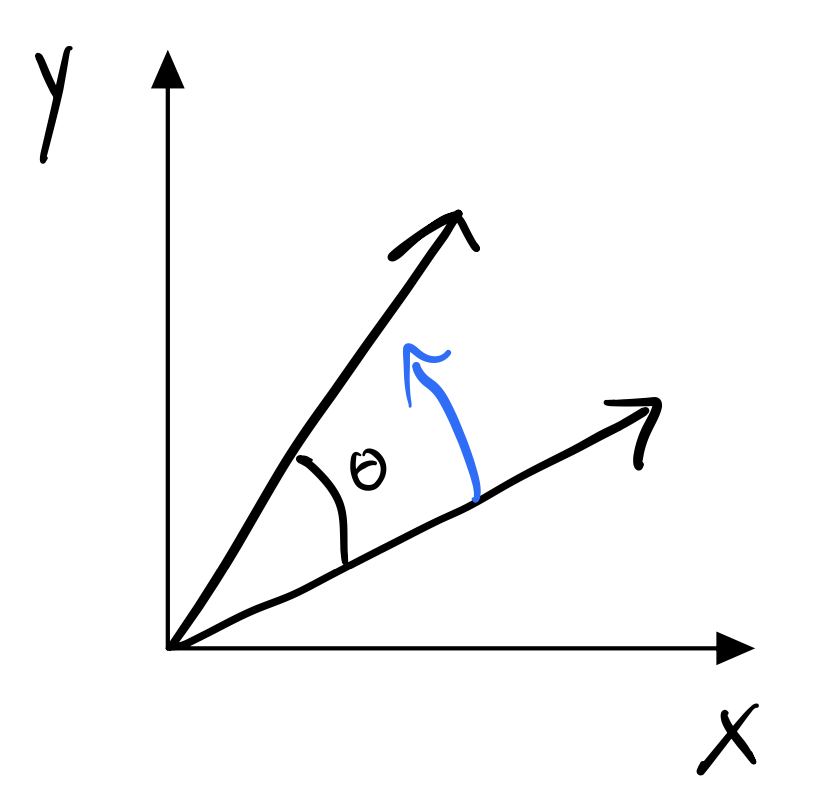
\includegraphics[scale=0.35]{Lectures/Images/lec2-rotation.png}
    \end{center}
    
\end{center}
we have:
\begin{equation}
    R = \m{\cos\theta & -\sin\theta & 0 \\ \sin\theta & \cos\theta & 0 \\ 0 & 0 & 1}
\end{equation}

For a boost in the $x'$ direction with velocity $v$, we have:
\begin{equation}
    \Lambda_{\mu}^{\sp\nu} = \m{\gamma & -\beta \gamma & 0 & 0 \\ -\beta \gamma & \gamma & 0 & 0 \\ 0 & 0 & 1 & 0 \\ 0 & 0 & 0 & 1}
\end{equation}
where the parameters obey (in order for $\Lambda$ to preserve the metric):
\begin{equation}
    \gamma^2(1 - \beta^2) = 1
\end{equation}
$\beta = \frac{v}{c} \in (-1, 1)$ as nothing travels faster than the speed of light. Rearranging for $\gamma$, we have the familiar expression:
\begin{equation}
    \gamma = \frac{1}{\sqrt{1 - \beta^2}}
\end{equation}

We can write:
\begin{equation}
    \beta = \tanh\zeta
\end{equation}
where $\zeta \in (-\infty, \infty)$ is the rapidity. In this parameterization:
\begin{equation}
    \gamma = \frac{1}{\sqrt{1-\beta^2}} = \frac{1}{\sqrt{1 - \tanh^2\zeta}} = \cosh\zeta
\end{equation}
where we have used $\cosh^2\zeta = \sinh^2\zeta + 1$. Note then that $\beta\gamma = \sinh\zeta$. So we can write the boost transformation as:
\begin{equation}
    \Lambda = \m{\cosh\zeta & -\sinh\zeta & 0 & 0 \\ -\sinh\zeta & \cosh\zeta & 0 & 0 \\ 0 & 0 & 1 & 0 \\ 0 & 0 & 0 & 1}
\end{equation}
Which looks quite analogous to what we had with the spatial rotations, except we have replaced the trigonometric functions with their hyperbolic counterparts. Indeed, we can view boosts as hyperbolic rotations.

Under a boost, we have:
\begin{equation}
    \m{x'^0 \\ x'^1} = \m{\gamma & -\beta\gamma \\ -\beta\gamma & \gamma}\m{x^0 \\ x^1} = \m{\gamma x^0 - \beta\gamma x^1 \\ \gamma x^1 - \beta\gamma x^0}
\end{equation}
In the nonrelativistic limit of $v/c \ll 1$:
\begin{equation}
    \gamma = (1-\beta^2)^{-\frac{1}{2}} \approx 1 + \frac{1}{2}\beta^2
\end{equation}
so:
\begin{equation}
    x'0 \approx x^0, \quad x'^1 = x' - \frac{v}{c}\cdot c t
\end{equation}
so we recover the expressions for old (Galilean) boosts. So classical physics was not wrong per se, it just emerges as the nonrelativistic limit of the correction theory. But when we look at relativistic physics (e.g. electromagnetic waves, high-energy particle scattering...) we need to use the relativistic theory.

On Tuesday, we discussed the 10 dimensional Galilean group which quantified the symmetry of classical mechanics. Now, we have modified boosts (i.e. the homogenous part of the Galilean group). The group consisting of 3 spatial rotations + 3 relativistic boosts yields the 6-dimensional Lorentz group, and the 4 spacetime translations yields the 10-dimensional Poincare group.

\subsection{Doppler Effect}
Recall the monochromatic wave solution:
\begin{equation}
    \phi = e^{ik_\mu x^\mu}
\end{equation}
with:
\begin{equation}
    k^2 = k_\mu k^\mu = 0
\end{equation}
\begin{equation}
    \omega = ck^0 = ck, \quad \v{k} = \hat{\v{k}}k = \hat{\v{k}}\frac{2\pi}{\lambda}
\end{equation}
The two heroes of the story are the frequency and $\hat{\v{k}}$ the direction of propagation.

\begin{center}
    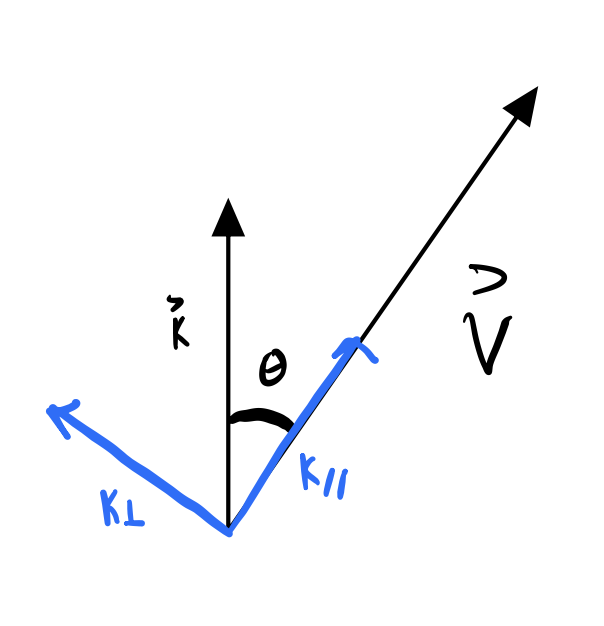
\includegraphics[scale=0.35]{Lectures/Images/lec2-wavevectorboost.png}
\end{center}

The question is now - what does a boosted observer see? We consider the wavevector $\v{k}$ and decompose it into the components perpendicular and parallel to the boost velocity. $\theta$ is the angle between the two vectors. Let us calculate:
\begin{equation}
    k'^\mu = \Lambda^{\mu}_{\sp\nu}k^\nu
\end{equation}
We have:
\begin{equation}
    k'^0 = \gamma(k^0 - \gv{\beta}\cdot\v{k}) = \gamma(k^0 - \beta k_\parallel)
\end{equation}
\begin{equation}
    k'_\parallel = \gamma(k_\parallel - \beta k^0)
\end{equation}
\begin{equation}
    \v{k}'_\perp = \v{k}_\perp
\end{equation}
the last equality follows from the fact that the $\Lambda$ matrix is trivial in this sector.

A good consistency check is that:
\begin{equation}
    k'^2 = k'_\mu k'^\mu = 0
\end{equation}
which you can verify. This tells us that the boosted observer still sees the EM wave propagating at speed:
\begin{equation}
    k'^0 = \abs{\v{k}'}
\end{equation}
This is not something to be surprised about - the formalism was built for this to be true.

If the speed of propagation is not different, what is different? Well, let's look at the $k'^0$ relation. We can write this as:
\begin{equation}
    \omega' = \gamma\omega(1 - \beta\cos\theta)
\end{equation}
So, we see a different frequency, which is the Doppler effect! The direction of propagation is also modified:
\begin{equation}
    \tan\theta = \frac{\abs{\v{k}_\perp}}{k_\parallel}, \quad \tan\theta' = \frac{\abs{\v{k}'_\perp}}{k'_\parallel} =  \frac{\abs{\v{k}_\perp}}{\gamma(k_\parallel - \beta k^0)}
\end{equation}
Since the denominator changes, so too must the angle.

Note the special case of the frequency relation when $\theta = \pi/2$, then:
\begin{equation}
    \omega' = \gamma\omega
\end{equation}
so the shift is manifestly relativistic.

\subsection{Teaser - Relativistic Formulation of Maxwell Theory}
You might say - hey, weren't we studying Maxwell theory the whole time? Indeed we were studying the wave equation, but there is more to Maxwell theory than this! We have to talk about two things:
\begin{itemize}
    \item The dynamics of (charged) particles in electromagnetic fields
    \item The dynamics of the electromagnetic field itself
\end{itemize}

Consider the Lorentz force; suppose we have particle with spatial coordinate $\v{x}(t)$ and charge $q$. In the presence of EM fields, the equation of motion is given by:
\begin{equation}
    \dod{(m\dot{\v{x}})}{t} = \dod{\v{p}}{t} = q(\v{E} + \v{v}\times\v{B})
\end{equation}
These equations are written in a highly inconvenient way for our purposes, as they treat time and space very differently. Time is a label and $\v{x}$ is the position of interest. But for us, we want to package things in terms of 4-vectors/spacetime coordinates $x^\mu = (x^0 = ct, \v{x})$. Thus the above formulation is very inconvenient, e.g., to see how Lorentz transformations work in this theory. We will see how we can formulate the Maxwell theory in a relativistically covariant fashion next time.